\documentclass[titlepage]{article}
\usepackage[utf8]{inputenc}
\usepackage[T2A]{fontenc}
\usepackage[russian]{babel}
\usepackage{gensymb}
\usepackage{amsmath,amssymb}
\usepackage{pict2e}
\usepackage{graphicx}
\title{Конспект по геометрии.}
\author{Каданцев Георгий, Коченюк Анатолий }
\date{13.01.2017}

\begin{document}
\maketitle
\setlength{\unitlength}{1cm}
\section{Формулы для вычисления площади}
    \subsection{Треугольник}
        \begin{itemize}
            \item[1.] По четвёртой аксиоме о площади площадь треугольника равна половине произведения длин одного из его оснований  на высоту, опущенной к нему:  
            $$\boxed{ S= \frac{1}{2}ah_a =\frac{1}{2}bh_b=\frac{1}{2}ch_c} $$
            \item[2.] Площадь треугольника равна половине произведения двух сторон на синус угла между ними.
            $$ \boxed{S=\frac{1}{2}ab\sin \gamma = \frac{1}{2}bc\sin \alpha = \frac{1}{2}ac \sin \beta} $$
            \item[3.] 
             Давайте найдём площадь треугольника, если известна длина одной его стороны и прилежащие к ней 2 угла. Обозначим сторону напротив одного из этих углов за $x$. По теореме синусов\\
             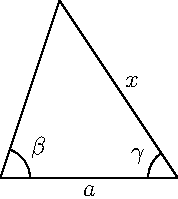
\includegraphics{pic_1o1.pdf}
            $$ x=\frac{a\sin \beta}{\sin (\beta+\gamma)} $$
            Следовательно 
            $$ \boxed{S = \frac{1}{2}ax\sin \gamma= \frac{1}{2}a^2\frac{\sin \beta \cdot \sin \gamma}{\sin (\beta +\gamma)}} $$
            \item[4.] Теперь найдём площадь треугольника, когда известны только 2 угла, назовём их $\alpha$ и $\beta$, и длина стороны напротив угла $\alpha$. Обозначим сторону напротив угла $\beta$ за $x$. По теореме синусов\\
             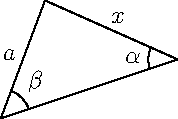
\includegraphics{pic_2o1.pdf}
            $$\frac{x}{\sin \beta}=\frac{a}{\sin \alpha}$$
            Откуда 
            $$ x = \frac{a \sin \beta}{\sin \alpha} $$ 
            $$ \boxed{S = \frac{1}{2}ax\sin (\alpha+\beta)=\frac{1}{2}a^2\frac{\sin \beta \sin (\alpha + \beta)}{\sin \alpha}} $$
        \item[5.] $$ S = \frac{abc}{4R} $$   
        $a$, $b$, $c$ -- стороны треугольника, $R$ -- радиус вписанной окружности.
        \item[6.] Рассмотрим произвольный треугольник и вписанную окружность. Проведём радиусы к точком касания и отрезки из вершин треугольника к центру окружности.
        \newline 
        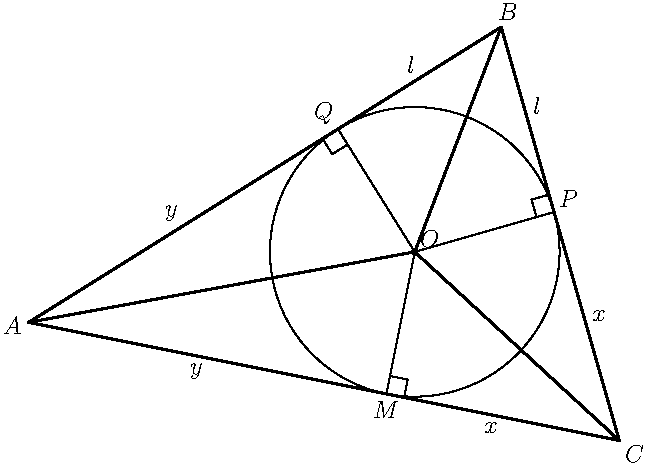
\includegraphics{incirc_2.pdf}\\        
        \setlength{\unitlength}{1cm}
        Теперь треугольник $ABC$ разрезан на треугольники $AOC$, $COB$ и $BOA$.
        Площадь этих треугольников обозначим за $S_1$, $S_2$ и $S_3$ соответственно.   
        $$\boxed{ S = S_1+S_2+S_3 = \frac{1}{2}br+\frac{1}{2}ar+\frac{1}{2}cr=
        \frac{1}{2}r(a+b+c)}$$
        
        \item[$6^*.$]
        Если в многоугольник можно вписать окружность, то площадь этого треугольника есть произведение полупериметра на радиус вписанной окружности.
        
        Рассмотрим такой многоульник. Он имеет n сторон, и будет разрезаться на n треугольников путём соединения вершин с центром окружности. Понятно, что доказательство в случае треугольника переносится.
        \newline
        \begin{picture}(5,5)
        \put(4,2){\circle{4}}
        \put(1,0){\line(1,0){5}}
        \put(1,0){\line(2,4.74){1.8}}
        \put(2.75,4.25){\line(9,-1.55){5}}
        \put(6,0){\line(2,1){1}}
        
        \put(4,2){\circle*{0.1}}
        
        \put(1,0){\line(4,2.65){3}}
        \put(2.8,4.25){\line(1.057,-2){1.2}}
        \put(6,0){\line(-1,1){2}}
        
        \put(0.36,0){\large{$A_1$}}
        \put(1.25,2.5){\large{$M_1$}}
        \put(2,4){\large{$A_2$}}
        \put(3.75,-0.48){\large{$M_n$}}
        \put(5.5,-0.48){\large{$A_n$}}
        
        \put(4,2){\line(-4.74,2){1.82}}
        \put(4,2){\line(0,-1){2}}
        
        \end{picture}
        \newline
        
        \begin{align*}
         S= S_1+S_2+S_3+\ldots +S_n =\\ \frac{1}{2}a_1r+\frac{1}{2}a_2r+\ldots +\frac{1}{2}a_nr= \\ \frac{1}{2}r(a_1+a_2+\ldots+a_n=\frac{1}{2}Pr=pr    
        \end{align*} 
         $$ \boxed{S=pr} $$
        $r$-- радиус вписанной окружности.
    \subsection{Прямоугольник}
       \item[7.] Любой прямоугольник любой диагональю делится на 2 равных треугольника.
       Так как эти треугольники прямоугольны, высота, опущенная на один из катетов совпадает с другим катетом.
        \newline
        \begin{picture}(4,2)
    \put(0,0){\line(1,0){4}}  
    \put(0,2){\line(1,0){4}}
    \put(4,0){\line(0,1){2}}
    \put(0,0){\line(0,1){2}}
    \put(2,0.12){\large{$a$}}
    \put(0.15,1){\large{$b$}}
    \put(0,2){\line(4,-2){4}}
    \put(0.25,0){\line(0,1){0.25}}
    \put(0.25,0.25){\line(-1,0){0.25}}
    \put(3.75,1.75){\line(0,1){0.25}}
    \put(3.75,1.75){\line(1,0){0.25}}
    \put(4.5,1){$\boxed{S=2S_{\triangle}=2\frac{1}{2}ab=ab}$}
    
    \end{picture}
    
   \item[8.] Площадь квадрата находится по формуле:
        $$ \boxed{S=a*a=a^2} $$
        \end{itemize}
    \subsection{Параллелограм}
        \begin{enumerate}
            \item $S=2*S_{\triangle}=2*\frac{1}{2}ab\sin\alpha= ab\sin\alpha$
            \item $S=2*S_{\triangle}=2*\frac{1}{2}ah_a=ah_a$
            \item $S =\frac{1}{2}d_1d_2\sin\alpha$\\
            $S=S_1+S_2+S_3+S_4=2S_1+2S_2=2*\frac{1}{2}xy\sin\alpha+2*\frac{1}{2}xy\sin\alpha=\frac{1}{2}d_!d_2\sin\alpha$
        \end{enumerate}
\end{document}
